\subsection{Hall Sensor}

There are two hall sensors implemented on the vehicle, one on each belt. A hall sensor is a sensor that is activated when exposed to a magnetic field. The sensors are placed beside the front wheels, on which there are four magnets, placed so that there is a quarter of a turn between them. The hall sensor is illustrated on \figref{HallSensor}.

 \begin{figure}[H]
	\centering
	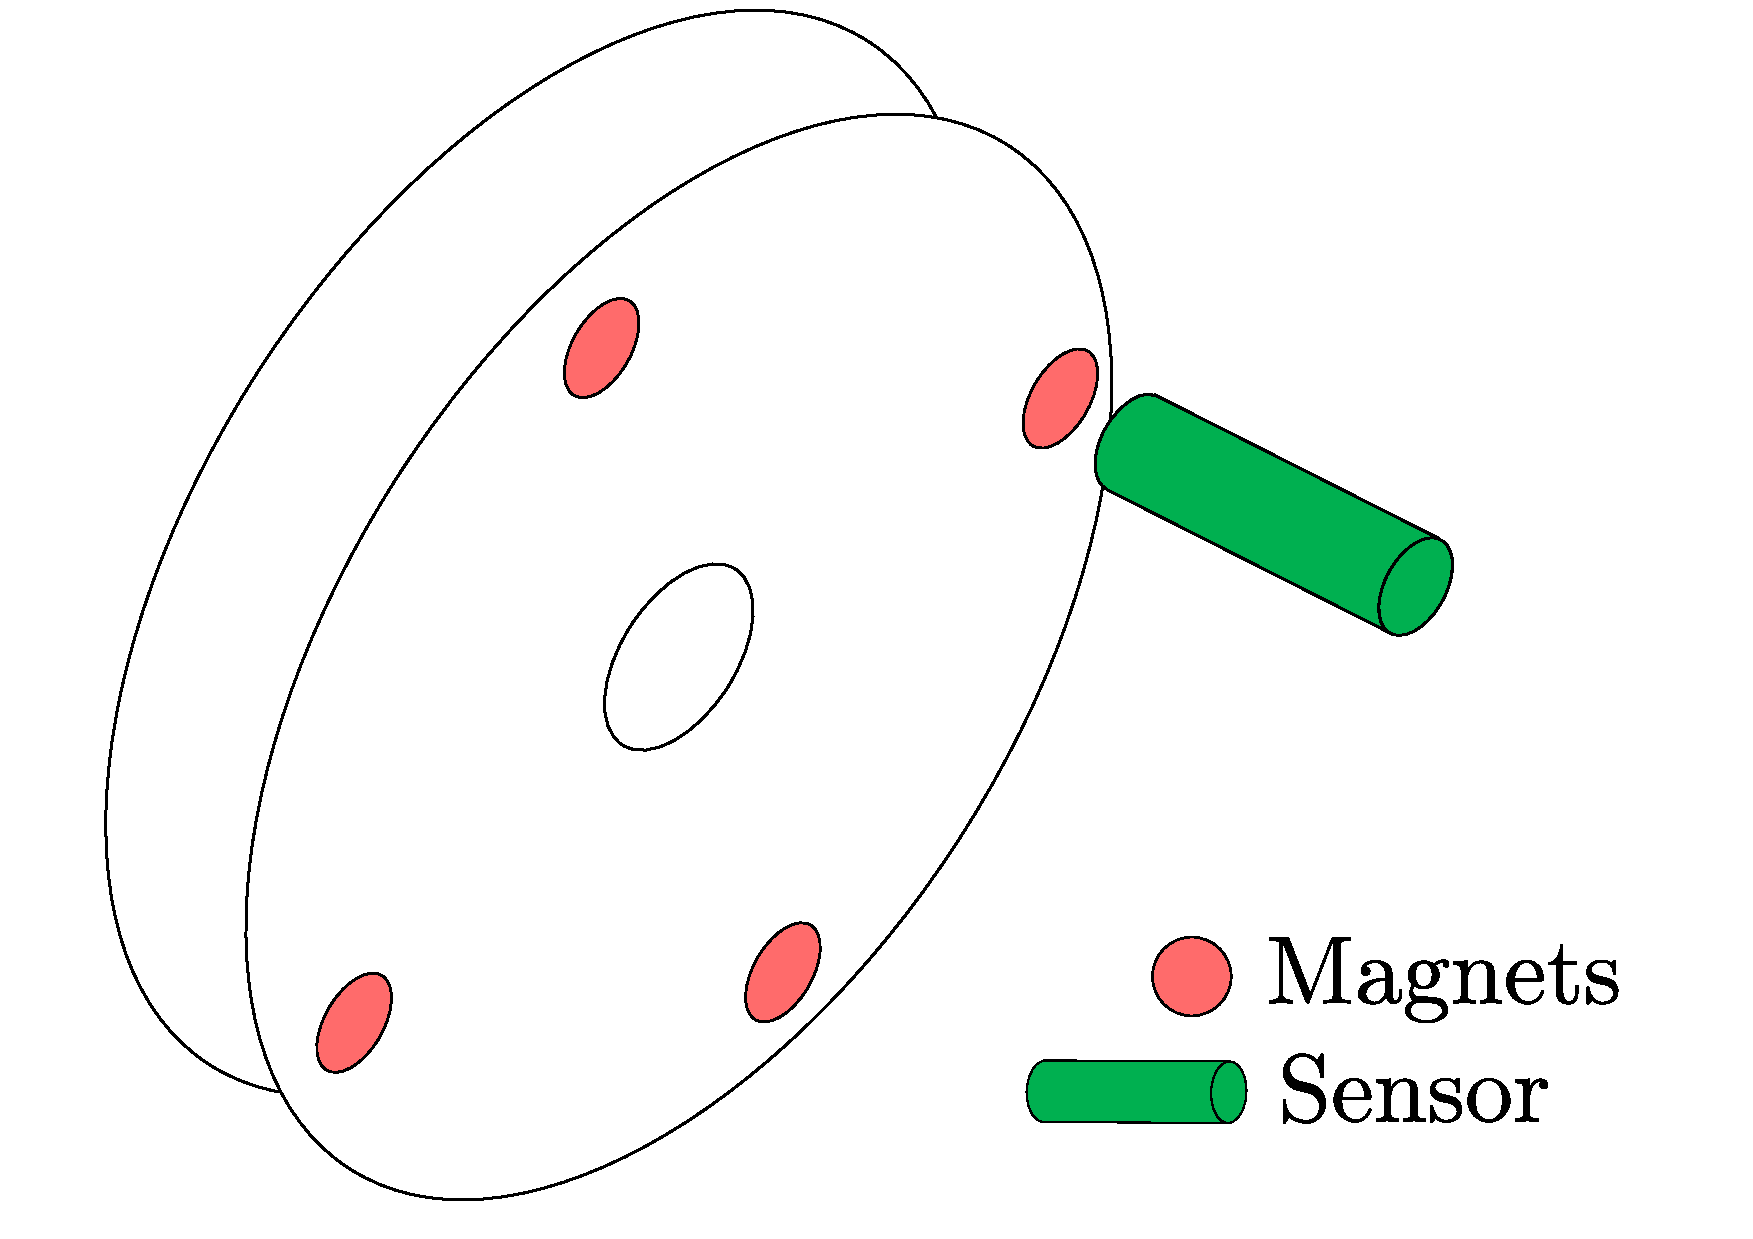
\includegraphics[scale=0.5]{figures/HallSensorSide_Forward_view.pdf}
	\caption{Illustration of the hall sensor, side view of the front wheel with magnets on, on the left and front view of the front view with the sensor, on the right. The red circles are the magnets and the green rectangle is the hall sensor.}
	\label{HallSensor}
\end{figure}

The Hall sensor will give a voltage output each time one of the magnets is in front of the hall sensor. This will give a signal each quarter of a turn of the wheel. Knowing the time a quarter of a turn will take by measuring the time between two outputs, and the distance that the vehicle travel on a quarter of a turn of the wheel, the speed of the vehicle can be calculated.

When the vehicle is starting to move, the first output from the hall sensor can not be used because of the random position of the wheel. The distance to reach the first magnet is not known. Therefore the speed can only be calculated by the second output.